%%%%%%%%%%%%%%%%%%%%%%% file sese_vorlage.tex %%%%%%%%%%%%%%%%%%%%%%%%%
%
% LaTex Beispiel für das Seminar Software Engineering.
% Enthält super interessante und wichtige Bearbeitungshinweise.
%
% Vorlage basiert auf der Springer LNCS Vorlage und ist nur
% für Seminararbeiten an der Universität Würzburg zu verwenden.
%
%%%%%%%%%%%%%%%%%%%%%%%%%%%%%%%%%%%%%%%%%%%%%%%%%%%%%%%%%%%%%%%%%%%


\documentclass[runningheads,a4paper]{uwsese}


%% -------------------------------
%% | Information for Declaration |
%% -------------------------------
\newcommand{\authorName}{Ștefan-Octavian Radu}
\newcommand{\place}{Würzburg}
\newcommand{\submissionTime}{28 February 2024}


\usepackage[utf8]{inputenc}
\usepackage{amssymb}
\usepackage{amsmath}
\setcounter{tocdepth}{3}
\usepackage{graphicx}
\graphicspath{ {./graphics/} }
\usepackage{array}
\usepackage{ragged2e}
\usepackage{arydshln}
\usepackage{xcolor}
\usepackage{parskip}
\usepackage[acronym]{glossaries}
\newcolumntype{P}[1]{>{\RaggedRight\hspace{0pt}}p{#1}}
%\newcolumntype{P}[1]{>{\raggedright\arraybackslash}p{#1}}

\usepackage{url}
\urldef{\mailsa}\path|dozent.ls2.informatik@uni-wuerzburg.de| 
\newcommand{\keywords}[1]{\par\addvspace\baselineskip
\noindent\keywordname\enspace\ignorespaces#1}

\makeglossaries
\newcommand{\newglossaryentrywithacronym}[3]{
    % From https://tex.stackexchange.com/questions/8946/how-to-combine-acronym-and-glossary
    %%% The glossary entry the acronym links to   
    \newglossaryentry{#1_gls}{
        name={#1},
        long={#2},
        description={#3}
    }

    % Acronym pointing to glossary
    \newglossaryentry{#1}{
        type=\acronymtype,
        name={#1},
        description={#2},
        first={#2 (#1)\glsadd{#1_gls}},
        see={[Glossary:]{#1_gls}},
    }
}

\newcommand{\newacro}[2]{
    \newglossaryentry{#1}{
        type=\acronymtype,
        name={#1},
        description={#2},
        first={#2 (#1)},
    }
}

\newglossaryentrywithacronym{CTF}{Capture the Flag}{ 
    In the context of security, CTFs are competitions where the participating teams attempt to exploit purpusefully vulnerable applications, in order to find text strings commonly known as ``flags'' and earn points
}

\newglossaryentrywithacronym{ELF}{Executable and Linkable Format}{ 
    ELF is a standardised file format, which originated in the Unix echosystem, used for binary executable files. It is adopted by multiple operating systems including: Linux, Solatris, BSDs, and many others \cite{corkami_elf}
}

\newglossaryentrywithacronym{CFG}{Control Flow Graph}{ 
    A CFG is a directed graph, modeling potential execution of a computer program. A set of maximal basic blocks (see \gls{BB}) constitutes the set of vertices. There is an edge in the graph between vertex $A$ and vertex $B$, if it is possible for the code associated with $B$ to be executed right after the execution of the code associated with vertex $A$ \cite{application_cfg}
}

\newglossaryentrywithacronym{ISA}{Instruction Set Architecture}{ 
    ``An Instruction Set Architecture (ISA) is part of the abstract model of a computer that defines how the CPU is controlled by the software. The ISA acts as an interface between the hardware and the software, specifying both what the processor is capable of doing as well as how it gets done.'' \cite{arm_isa}
}

\newglossaryentrywithacronym{BF}{Brainf*ck}{ 
    Brainf*ck is a very famous esoteric programming language, known for its minimalis syntax which consists of only the following eight instructions: \cc{+ \_ < > . ; [ ]}
}

\newglossaryentrywithacronym{IR}{Intermediate Representation}{ 
    An IR is an abstract, fully encompassing, structure capable of expressing the operations which can be performed on a target (virtual) machine. IRs are commonly used during the compilation process, in order to facilitate further transformations \cite{ir_compilers}
}

\newglossaryentrywithacronym{BB}{Basic Block}{ 
    A basic block is a (typically) maximal sequence of instructions that ``are guaranteed to execute together''. Any branch incoming to a basic block will end at its entry point. Any branch outgoing from a basic block will start from its exit point \cite{application_cfg}
}

\newacro{CC}{Command and Control}
\newacro{SE}{Symbolic Execution}
\newacro{RE}{Reverse Engineering}
\newacro{CE}{Concrete Execution}
\newacro{PI}{Propriatery Information}
\newacro{SOTA}{State of the Art}
\newacro{VM}{Virtual Machine}
\newacro{NSA}{National Security Agency}
\newacro{UI}{User Interface}
\newacro{stdin}{standard input}
\newacro{IP}{Instruction Pointer}
\newacro{SP}{Stack Pointer}
\newacro{syscall}{System Call}
\newacro{OS}{Operating System}
\newacro{CLE}{CLE Loads Everything}
\newacro{CPU}{Central Processing Unit}
\newacro{SMT}{Satisfiability Modulo Theories}
\newacro{DSE}{Dynamic Symbolic Execution}
\newacro{MBA}{Mixed Boolean-Arithmetic}


\begin{document}

\mainmatter 

% first the title is needed
\title{Trusted Execution Environments: An Overview}
\subtitle{Software Engineering Seminar}

% a short form should be given in case it is too long for the running head
%\titlerunning{Bearbeitungshinweise Seminar Software Engineering}
%\titlerunning{} %TODO

\date{Winter Semester 2023-2024}


\author{Ștefan-Octavian Radu}
%
%\authorrunning{LS2 Dozent}
%\authorrunning{Trusted Execution Environments: An Overview} %TODO
% (feature abused for this document to repeat the title also on left hand pages)

% the affiliations are given next
\institute{University of W\"urzburg,
Germany\\
\mailsa\\
}

\maketitle

\begin{abstract}

    With computing systems processing more and more information, arose the need
    for more rigorous security guarantees for the processed data. \gls{TEE} are
    one of the solutions which addresses the problem of secure computation. They
    enable secure code execution and data storage in a secure isolated
    execution environment. In this paper we will cover the architecture of
    these systems, how they are currently used both in the industry and in
    academia, and what tools are available for application development. In the
    end we will cover some known attacks that have been proven to compromise
    the security guarantees of \glspl{TEE}.

\end{abstract}

% Intro {{{

\section{Introduction}

Currently, computers and computing systems have reached a very high level of
complexity. As a result, the solutions for securing such systems are inherently
difficult to find. The risk of security breaches in critical infrastructure is
increasingly higher as its complexity increases. That is why, proposals related
to isolated execution environments that can guarantee the secure computation of
security-critical applications, are only natural.

A pertinent solution which addresses the problem of secure computation in
security-critical applications is the adoption of \glspl{TEE} for enhancing the
threat-protection on a vast range of computing devices, from end user mobile
devices to cloud systems. The goal of \glspl{TEE} is to offer superior
security guarantees. This is achieved by enforcing a strong barrier between
execution through an operating systems and secure execution and data storage
through a \gls{TEE}. In this way \glspl{TEE} address the issue of trust, moving
trust from complex systems which are hard to prove secure and have been
subject to many security breaches in the past, to a small set of security
primitives which enable the creation of isolated execution environments with
considerably smaller attack surfaces.

By combining information from multiple sources, we get a definition as
follows. A \gls{TEE} is a feature of modern microprocessors which provides a
hardware-isolated ``secure area that runs in parallel with, but separate, from
the normal execution environment'' \cite{tee_ieee_standard}. This environment
aims to guarantee that the executed code, the runtime states and the stored
data are integrity and privacy protected. It's end goal is to improve the
overall security of the whole system, by enabling the safe execution of
security-critical applications (\cite{tee_app_rev}, \cite{tee_in_securities},
\cite{tee_is_and_not}).

In this paper we will give an overview of \glspl{TEE}. We will start by
discussing in detail the architecture and the security principles that
\glspl{TEE} are based on, in order to facilitate a deeper understanding of the
technology and a knowledge base for the following sections. This section will
cover chains of trust from initialisation until the instantiation of an
\gls{enclave}, memory protection of various components during runtime, the
secure storage of information across enclaves and how secure interaction with
external IO devices can be performed. Next, we will cover the main applications
of a \gls{TEE}, the array of tooling available for the development of
applications for \glspl{TEE} as well as common difficulties currently faced as
part of the development process. Lastly, we will highlight some security
shortcomings of this technology, by discussing the main classes of security
vulnerabilities which have been found to affect \glspl{TEE} since their
adoption. In this section we aim to emphasize the fact that security enhancing
technologies are beneficial, but often not perfect, which leaves room for
further improvements in the future. We will end the paper with a list of
acronyms and a glossary with relevant terms.

% }}}

% HW TEE {{{

\section{Hardware-based \gls{TEE}}

There has been a lot of research and development effort put into \glspl{TEE} in
the recent years. The most common types of \gls{TEE} are based on
architecture-specific hardware extensions which enable the creation of
enclaves. These will be the focus of this section. There are both commercial
and academic solutions implemented, spanning across all major computer
architectures (Intel, AMD, ARM, POWER, RISC-V) and even more niche ones (SPARC,
OPEN-RISC). It has been shown in a previous survey that despite different
approaches in design, there are four security principles common among all
implementations: \emph{verifiable launch}, \emph{run-time isolation},
\emph{secure storage}, \emph{trusted IO} and \emph{secure storage}
\cite{tee_hw_sup}. An \emph{non-general} overview of these building blocks can be
visualised in Figure \ref{fig:tee_components}.

\begin{figure}[h]
    \centering
    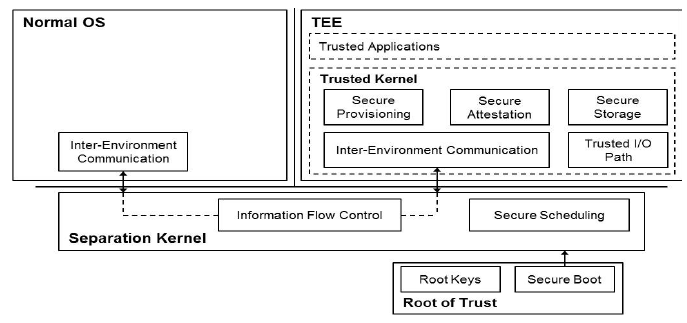
\includegraphics[scale=.7]{tee_components.png}
    \caption{An overview of \gls{TEE} building blocks \cite{tee_is_and_not}}
    \label{fig:tee_components}
\end{figure}

\subsection{Verifiable Launch}

Before the enclave is even launched into execution, an important first step
must be accomplished. \emph{Verifiable launch} aims to ensure that the initial
state of the environment matches its expected state. It must also confirm that
the initial configuration is correct. 

\subsubsection{Root of Trust (Measurement).}
\label{rot}

The base of this process is an entity called \emph{\gls{RTM}}. This is the
anchor of trust for the process of measurement, thus it is assumed to be secure
by design. In this context, trust is defined as the property of a system to
match its expected state of being secure. There are three types of \glspl{RTM}
used by \glspl{TEE}:

\begin{itemize}
    \item \gls{SRTM} (TCG \cite{tee_tcg_arch_overview}, Secure Boot
        \cite{windows-driver-content2023Dec}) is obtained through an
        uninterrupted \emph{chain of trust} from boot time (reset) until the
        first line of code that runs in the enclave. The chain of trust will
        generally include all software in the \gls{TCB}, but not the OS (as it
        is considered untrusted software by default). It can be implemented in
        hardware directly, or as immutable software. The downside of \gls{SRTM}
        is that it cannot guarantee anything about the state of the system
        mid-runtime, because it can be subject to cyberthreats after boot
        \cite{tee_smart_rot} \cite{tee_hw_sup}.
    \item \gls{DRTM} runs without trusting any prior execution. It is based
        on various architectural extensions that are meant to protect against
        adversaries that may exist on the system upon the start of the enclave.
        After all active processes are suspended and IO devices are disabled, a
        signed module is loaded, measured and authenticated. This will serve as
        the \gls{TCB} and will be responsible for loading and measuring future
        enclaves \cite{tee_hw_sup}.
    \item Hardware RTM (HW) can attest that a software module is not tampered
        and can be securely executed, without relying on any software. It is
        not a common implementation, but proposals such as Sancus
        \cite{tee_sancus}, or Iso-X \cite{tee_isox} exist. 
\end{itemize}

Out of the 31 implementations analysed in the survey, only a few of them
implement \gls{DRTM}, some of them being commercial solutions from Intel and
ARM (\cite{arm_tz}, \cite{intel_tdx}, \cite{intel_sgx}). The rest, and the vast
majority of the academic solutions, use variants of \gls{SRTM}. Only one
proposal uses HW.

\subsubsection{Measurement.}

Regardless of design, each RTM involves a trusted chain of execution, where
each component \emph{measures} the next one in the chain, before passing on
execution. The measurement process consists of building a chain of
cryptographic hashes that are then securely stored. Components in the chain
are, in practice, also integrity checked \cite{tee_hw_sup}. This process is
typically done in a mutable part of the software \gls{TCB} with only a few
exceptions \label{hw_exp} such as Sancus \cite{tee_sancus} and Iso-X
\cite{tee_isox}.

\subsubsection{Attestation.}

\emph{Attestation} is the process of ensuring that upon the launch of the newly
created enclave, its state, measurement, and its whole \gls{TCB} correspond to
their reference values. This is done by a \emph{verifier}, which splits the
process into: \emph{local attestation} and \emph{remote attestation}, based on
the location of the verifier. They usually differ by the method of encryption
used, the remote verifier commonly using \emph{public key cryptography}, while
a verifier co-located with the enclave will use \emph{symmetric key
cryptography}, which is lighter on resources. Most of the analysed solutions
use remote attestation, and only a few of them also support local attestation,
concluding thus that remote attestation is the standard both in industry and in
academia \cite{tee_hw_sup}. Like measurement, attestation is also done in
software with the same few exceptions seen in \ref{hw_exp}.

\subsubsection{Provisioning.}

\emph{Provisioning} secrets into the newly created enclave is an optional step
that can be performed and is usually done either as a last step, or before the
attestation. In case the provisioning is performed before the attestation, the
measurement will also reflect the inclusion of the secrets. \cite{tee_hw_sup}

\subsection{Run-Time Isolation}

The resources used by the enclave during its runtime must be protected against
tampering, or reading by adversaries. These resources include the \emph{CPU}
and \emph{memory}. As noted in \cite{tee_hw_sup}, we can categorize
run-time isolation by the method of \emph{partitioning} resources into a scale
from \emph{spatial} partitioning to \emph{temporal} partitioning. Extremes are
unusual, so a middle ground called \emph{spatio-temporal} partitioning is a
common choice. Isolation enforcement is categorised into \emph{logical
isolation} and \emph{cryptographic} isolation.

\subsubsection{CPU isolation.}

When analysing these strategies for \glspl{CPU} it has been noted that the
majority are suboptimal. Spatial separation would involved dedicating \gls{CPU}
cores to specific enclaves, which would inherently limit the total number of
possible simultaneous enclaves. A mixed, spatio-temporal solution is also
sub-optimal because of implementation difficulties. This solution would require
extra hardware in order to guarantee the integrity of spatially-separated
resources. On the other side, cryptographic enforcement would incur large
computational overhead and would likely require extra hardware. With these
considerations, the optimal solutions for \gls{CPU} isolation would be the
logical enforcement of a temporal partitioning \cite{tee_hw_sup}.

The analysis shows this is indeed the case with all analysed \gls{TEE}. This is
achieved through secure context switching during which the state of the enclave
is saved, the registers of the \gls{CPU} are cleared and the state of the next
enclave is loaded. The \emph{\gls{TCB}} is responsible for this process and
must ensure that there is no data leakage during the context switch. To achieve
a secure context switch the \emph{\gls{TEE}} relies on a combination of
\emph{privilege levels} and \emph{architectural extensions}. Most commercial
solutions have introduced new processor execution modes in support of
\glspl{TEE}: Intel SGX - \emph{Enclave mode} \cite{intel_sgx}, Intel TDX -
\emph{SEAM mode} \cite{intel_tdx}, ARM CCA - \emph{Secure Mode} \cite{arm_cca},
IBM PEF - \emph{Secure Mode} \cite{ibm_pef}. Academic solutions take a
different approach, and rely on firmware running at a higher privilege level.
To ensure that the \gls{TCB} can implement the necessary security mechanisms
needed (attestation, measurement, isolation, etc.) it usually runs at higher
privilege levels, compared to the \gls{TA} or \gls{VM} that run in the enclave,
typically at lower privilege levels \cite{tee_hw_sup}. 

\subsubsection{Memory Isolation.}

This is a very challenging task as part of a \gls{TEE} architecture, because it
involves protecting not only the memory itself, but also various
micro-architectural structures holding recent code, branch predictions, or
recent instructions. Another important consideration is the implementation of
virtual address translation into physical addresses.

By employing the same categorisation criteria, it's been observed that
successful \gls{TEE} implementations use a diverse range of partitioning
strategies. Spatial partitioning implies assigning at system boot an area of
memory to be used only by enclaves or the \gls{TCB}, which works well for a low
number of enclaves which have static and predictable memory requirements.
Spatial partitioning is also often leveraged to protect access control
information. Temporal isolation is the most rarely used strategy, because the
context switching is very computationally expensive, making it not suitable for
systems running concurrent enclaves. The preferred solution is the mixed
spatio-temporal partitioning as it enables dynamic reallocation of partitions
based on runtime requirements. Logical enforcement of isolation is based on an
\emph{access control mechanism} \label{acc_control} to only give access to
trusted entities. Integrity can be achieved efficiently and requires minimal
information for each enclave. Cryptographic enforcement is very strong in the
sense that it ensure confidentiality, integrity and can protect against
\emph{replay attacks} \cite{tee_replay_attacks}. However, they come at the cost
of higher storage and computation overhead, which makes it hard to scale.
Distinctly from the other isolation strategies, cryptographic isolation can
counter an adversary which leverages specialised hardware to perform a
\emph{man in the middle} attack at the \gls{BUS} level \cite{tee_hw_sup}
\label{bus_crypto}.

In practice, there are clearly preferred paths of implementation. Most
solutions use logically enforced spatio-temporal isolation for enclave memory
and logically enforced and exclusively spatial isolation for the \gls{TCB}. As
stated earlier, there are also implementations that use different strategies.
\emph{Flicker} \cite{flicker} and \emph{SEA} \cite{sea_minimal_tcb} use
logically enforced temporal isolation for both the enclave memory and the
\gls{TCB}. Among others, SEV \cite{amd_sev} by AMD and AEGIS \cite{aegis}, use
cryptographically enforced spatio-temporal isolation for the enclave's memory.
The latter uses the same strategy for isolating the \gls{TCB}. All sampled
implementations, however enforce the isolation via cryptographic means at the
BUS level \ref{bus_crypto}.

\subsubsection{Architectural details of memory isolation.}
\label{sect:mem_isolation}

Logical enforcement of spatio-temporal isolation is achieved through
\emph{access control mechanisms} as seen in \ref{acc_control}. The surveyed
\gls{TEE} use either \gls{MPU} or \gls{MMU}. \glspl{MPU} check access rights
against physical addresses of memory and can typically offer coarse-grained
memory control. This is achieved by enforcing a limited set of access control
rules, which must be managed by the \gls{TCB}. \glspl{MPU} are preferred in
academic solutions and are seen in modern \gls{TEE} such as Sancus
\cite{tee_sancus}, Keystone \cite{tee_keystone}, or CURE \cite{tee_cure}.
\glspl{MMU} offer more fine grained control. \glspl{MMU} handle virtual
addresses and convert them to physical addresses via page tables. Entries in a
page table also hold sensitive information which must be protected (eg. access
permissions). This is achieved either by letting the \gls{TCB} manage all page
tables of the enclaves as well as the page tables of all \emph{untrusted
software} \cite{tee_ha-vmsi}, or by having the \gls{TCB} manage only the tables
of the enclaves and then using additional access information for enclave
access, based on the execution context \cite{intel_tdx}, \cite{arm_tz},
\cite{arm_realms} \cite{tee_hw_sup}.

\subsubsection{Caches.}

Caches store recently accessed data to improve performance. Caches have also
been notoriously used for leaking data, as will be further seen in
\ref{cache_attacks}. Enclave data can be protected in the cache by using
functions of the \gls{MMU} / \gls{MPU}, as seen in some architectures
\cite{intel_sgx}. In other architectures this is achieved with additional
protection strategies \cite{arm_tz}. Most of the solutions involved logically
enforced spatio-temporal isolation of the caches, but there are exceptions,
mainly aiming to mitigate \gls{SCA} \ref{sidechannel_attacks}. Spatial
partitioning, despite not scaling well and diminishing performance is
implemented for example in MI6 \cite{tee_mi6}, or Keystone \cite{tee_keystone}.
Temporal partitioning involves flushing the full cache on each context switch,
which drastically degrades performance, but from the same prior considerations
it is used in a few implementations such as SANCTUARY \cite{tee_sanctuary}, or
Sancus \cite{tee_sancus}. No cryptographic solution for isolation has been used
for caches, most likely because of the considerable increase in latency it
would result in \cite{tee_hw_sup}.

\subsection{Secure Storage}

\emph{Sealing} is defined as the process of protecting state data across
different instances of the same enclave, through encryption. \emph{Unsealing}
is the opposite of sealing.

As a result of the survey, it's been determined that all \gls{TEE} solutions
that explicitly describe their design choices for secure storage follow closely
the sealing algorithm of the \gls{TPM} \cite{trust_plat_mod}, an immutable
hardware component. An asymmetric key pair used to encrypt a secret. The secret
will only be unsealed if the system state matched the state at the time of
sealing. Further, the secret is used for decrypting the stored data. Solutions
such as SEA \cite{sea_minimal_tcb}, or IBM-PEF \cite{ibm_pef} are based on a
\gls{TPM} microcontroller. Intel SGX \cite{intel_sgx} exposes sealing
capabilities through \gls{CPU} instructions. There are however, solutions which
provide sealing support purely thought their software \gls{TCB}, such as
\cite{optee}, or \cite{tee_timber}. This is useful in solutions which utilise a
software \gls{TCB}, as it it not dependant on the system's hardware
\cite{tee_hw_sup}.

\subsection{Trusted IO}

In the context of \glspl{TEE}, \emph{Trusted IO} refers to the secure
interaction between enclaves and external devices. It has two components:
\emph{trusted path}, and \emph{trusted device architecture}.

\subsubsection{Trusted Path.}

A \emph{trusted path} is a secure communication channel that ensures
confidentiality and integrity of enclave's access to the device. It can be
established either through logical or cryptographic means.

Logical trusted paths require architectural support for \gls{DMA} and
\gls{MMIO}. The former involves the same techniques used to protect memory
access in an enclave (see \ref{sect:mem_isolation}). A trusted path for \gls{MMIO}
can be implemented by allowing or denying \gls{MMIO} requests based on source
or destination. This can be achieved through access filters. A number of
implementations leverage the \emph{Trusted Protection Controller} from ARM for
this task \cite{tee_truz_droid}, \cite{tee_vbutton}. Solutions such as CURE
\cite{tee_cure} and HECTOR-V \cite{tee_hector_v} use more complex filters
before each IO device. As seen in \ref{sect:mem_isolation}, \glspl{MPU} can be used
to create secure memory mappings, which can be used to build trusted paths
between enclaves and IO devices.

Cryptographic trusted paths are based on encryption and create a secure
communication channel between the enclave and the device, which must be both
provisioned with credentials and cryptographic keys for authentication. As
previously mentioned, these solutions come with a computational overhead, but
can also bring the advantage of protection at the \gls{BUS} level. There are a
number of \glspl{TEE} which utilise cryptographic trusted paths either solely
(eg. HIX \cite{tee_hix}), or in combination with logical trusted paths (eg.
SGXIO \cite{tee_sgxio}).   

\subsubsection{Trusted Device Architecture.}

There are some devices which do not process confidential data in clear text for
which only a \emph{trusted path} is suffices. However, there are are devices
that gained traction in the last few years which make computations on user
data, and which must ensure confidentiality and integrity of this data.
Examples of such devices are GPUs, dedicated AI chips, or FPGAs. Since the
devices differ significantly in architecture, only a high-level overview of the
implementation strategy could be covered \cite{tee_hw_sup}. Temporal
partitioning of the IO device is a common strategy and requires a secure
context switch. Examples include HEETEE \cite{tee_heetee} for generic
accelerators, HIX \cite{tee_hix} for GPUs and ShEF \cite{tee_shef} for FPGAs.
Logically enforced temporal partitioning is also a common solution when
multiple enclaves need to access a resource concurrently. This is typically
achieved through an architecture specific mechanism of partitioning resources
to enclaves and keeping track of ownership. Recent proposals include SEGIVE
\cite{tee_segive} for GPUs and TrustOre \cite{tee_trustore} for FPGAs. Spatial
partitioning and cryptographic enforcement are considered unsuitable
\cite{tee_hw_sup}.

% }}}

% Other Architectures {{{

\section{Other Architectures}

The vast majority of relevant academic and industry \gls{TEE} implementations
used hardware extensions to provide the necessary building blocks for
\gls{TEE}. There exist however some architectures that diverge from this trend.

Purely software-based architecture try to address the dependence of \glspl{TEE}
on the \gls{CPU} architecture of the system they are running on. A relevant example
is SecTEE, which implements in its software \gls{TCB} all primitives necessary
for running secure enclaves: ``integrity measurement, remote attestation, data
sealing, secrets provisioning, and life cycle management'' \cite{sec_tee}.

On the other hand, we find solutions such as AMD Platform Security Processor
(PSP), Google Titan M, Apple Secure Enclave Processor (SEP) or Hardware
Security Modules (HSM), which aim to provide similar benefits with \gls{TEE},
but are implemented as separate chips from the main \gls{CPU}.

% }}}

% Applications {{{

\section{Applications \& Developer Support}

This section is based on a recent study by Paju et al. \cite{tee_app_rev} where
they analyse the recent evolution of \gls{TEE} usage both in academia and in the
industry. The main topics covered in the survey include application use-cases,
\gls{SDK}, trusted containers and their performance.
There are also a number of insightful tables covering usage-example graphs,
application classification in groups, development tools and trusted container
support that were not included in this work, but could be inspected in the
original paper.

\subsection{Applications of \gls{TEE}}

Research shows that the number of applications that utilise \gls{TEE} has been
increasing since 2015. Out of the surveyed use cases, the majority of the
deployed application are open-source. This stems most likely from the absence
of documentation and scholarly studies of proprietary application.

The vast majority of the surveyed applications run on platforms backed by Intel
SGX \cite{intel_sgx}, ARM TrustZone \cite{arm_tz}, or both. Only a minority run
on AMD SEV \cite{amd_sev}, RISC-V \cite{tee_keystone}, or GPU TEEs. Use cases
can be separated in various categories as follows.

\subsubsection{Data Analysis and Cloud.} 

The main applications used for data processing are based on \gls{ML}. This is
especially prevalent with the rise of AI and with its success in the healthcare
and financial industry. Often, \gls{ML} applications process sensitive
information which can be protected through the use of \glspl{TEE}. Moreover,
cloud computing is frequently used for \gls{ML} applications. In the context of
the cloud, \glspl{TEE} can provide protection against compromised
infrastructure, isolating crucial data and code from adversaries. Both \gls{ML}
applications and cloud computing make up the two largest categories of
\gls{TEE} usage.

\subsubsection{Finance and Authentication}

Grouped here are smaller categories, that together add up to a relevant number
of applications. These include various use cases related to online payments,
such as mobile wallets, cryptocurrency wallets, peer-to-peer (P2P) payments, or
applications enabling a mobile device to be used as a point-of-sale terminal.
\gls{TEE} have been proved to be useful in protecting the privacy of
lightweight blockchain clients, without affecting performance
\cite{light_blockchain}.

\gls{TEE} are also commonly used for a wider range of authentication methods
(fingerprint scanning, facial recognition, voice recognition), especially in
mobile devices \cite{tee_in_android}. Biometric identification data has been
protected, by being stored in a \gls{TEE}. Recently however, there has been an
increase in solutions that process and verify biometric data directly on the
sensors. Even in such cases, \gls{TEE} are still used to share the attestation of
the biometric data. Cryptographic private keys are another example of critical
data stored in \glspl{TEE}. Solutions such as Apple's \emph{passkey}
\cite{apple_passkey} use both cryptographic primitives and biometric
information to enable password-less authentication.

\subsubsection{Security Solutions}

There are many security solutions based on \gls{TEE}. Examples include remote
attestation systems, solutions for secure code offloading to IO devices, such
as GPUs, secure storage solutions, network security (TOR enhancements, trusted
execution of JS, publish/subscribe systems), secure channels (between \gls{TA} and
REE or peripherals which can be remote or local) and content sharing, primarily
digital rights management (DRM) \cite{tee_app_rev}.

\subsubsection{Others}

Other use cases include smart contracts, computer games, medical data, formal
methods, accelerators, or niche implementations of web searches protection, 
digital contract signing, or secure logging \cite{tee_app_rev}. A visual overview
of the most relevant application categories and related security properties can be
seen in Figure \ref{fig:tee_apps}.

\begin{figure}[h]
    \centering
    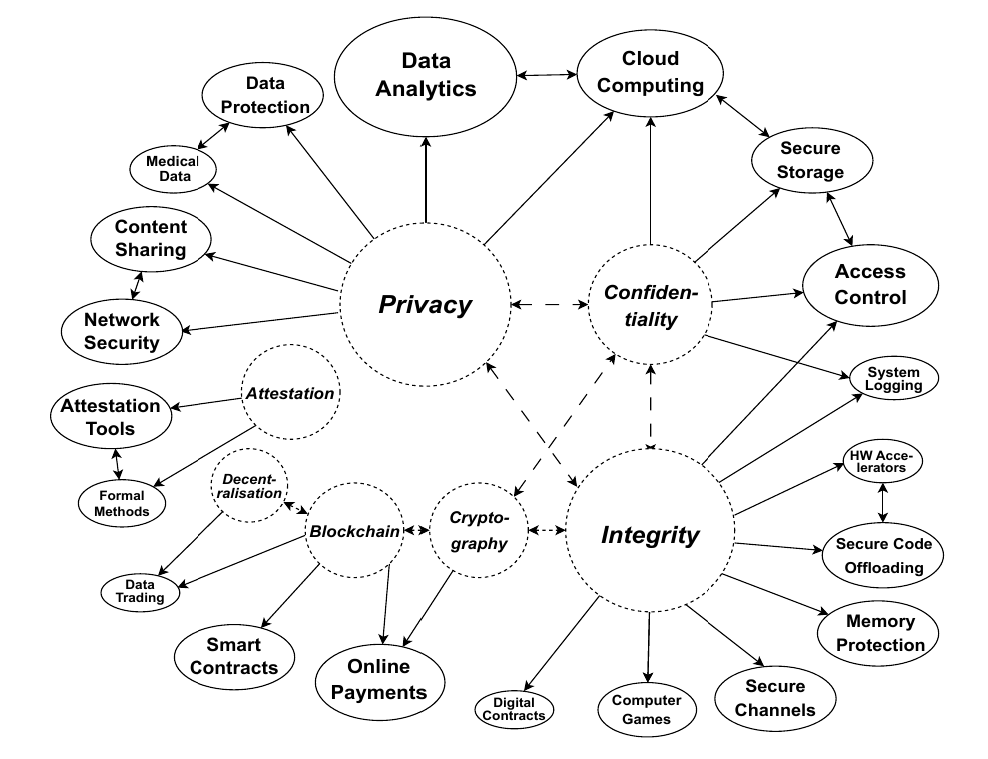
\includegraphics[scale=.43]{tee_apps.png}
    \caption{An overview of the most common \gls{TEE} application use cases and
        related security properties \cite{tee_app_rev}}
    \label{fig:tee_apps}
\end{figure}

\subsection{Application Development}

There are a number of available \glspl{SDK} development process of \gls{TA}. The majority of the surveyed \glspl{SDK},
support either Intel SGX, or ARM TrustZone, namely ``21 of the 23 referred
frameworks''\cite{tee_app_rev}. There are also two development tools which
offer support for RISC-V, namely Keystone \cite{tee_keystone} and Sanctum
\cite{tee_sanctum}, the latter of which appear to not be in development any
longer. With regards to programming language support, the vast majority support
either C or C++, but there are some exceptions. OP-TEE \cite{optee} also offers
support for Rust, among others like Edgeless RT \cite{edgelessrt} which also
supports Go. The Samsung Knox \gls{SDK} \cite{knox_sdk}, but also open source
projects like Trusty TEE \cite{trustytee} offer Java support for the
development of Android apps.

Developers are restricted in their choice of \gls{SDK} by the platform they're
developing for. Most Android TEE-enabled devices use ARM chips, and will thus
need a solution designed for \gls{TZ} \cite{arm_tz}. This resulted in
developers being constrained to use proprietary tools such as Samsung Knox \gls{SDK}
\cite{knox_sdk}. However, frameworks such as OP-TEE \cite{optee} and Trusty TEE
\cite{trustytee} might be viable open source alternatives for mobile
application development. Despite the many open-source options available, their
platform support, is yet limited.

\subsection{Trusted Containers}

Adapting an application to run inside a \gls{TEE} requires a lot of development
effort for making framework-specific changes. Generally, frameworks are
architecture specific. This, in turn, means that supporting a \gls{TA} on
multiple architectures is a very difficult task. \gls{TCON} aim to bridge this
gap in \gls{TA} development. \glspl{TCON} come in as solutions which either
enable an application to run unmodified inside a \gls{TEE}, or enable automatic
code modification of the application, such that it can run in the \gls{TEE}.
The downside of \glspl{TCON}, from a security perspective, is that they
increase the \gls{TCB}. From a development standpoint however, the trade-offs
could be worth it, considering the lower amount of resources invested in
porting the application to run on a \gls{TEE} and the fact that some
applications have a limited amount of system interactions (eg. \gls{ML} models)
which, as a result, diminishes their attack surface. A non exhaustive list of
the surveyed \glspl{TCON} include: Twine, Gramine, vSGX, Apache Teaclave and
Occlum. 

Out of all the containers analysed, none support \gls{TZ}, which further
confines mobile developers to using \glspl{SDK}. Intel SGX is the most supported
architecture with 19 out of 20 projects supporting it. Only a few of them also
support AMD SEV. There are recent solutions which offer support for both
platforms, such as vSGX \cite{vsgx}. Such solutions can further simplify
development by enabling an application to run unmodified on different \gls{TEE}
architectures.

LibOS \cite{libos} is a solution which was first used ten years before the
concept of \glspl{TEE} first emerged. Its purpose is to be an intermediary
between the OS and the client, by exposing OS functionality through a set of
libraries. LibOS is useful in the context of \gls{TEE} and \glspl{TCON}
especially, because Intel SGX restricts system calls inside the enclave.
Because of that, unmodified applications cannot run inside an SGX enclave.
Through LibOS however, system calls from inside the enclave can be securely
relayed to the OS outside of the enclave. There are further advantages of using
LibOS such as smaller \gls{TCB} as a result of OS encapsulation and increased
performance as a result of a reduction in context switches.

Wrappers around the libc library, or the \gls{WASI} act similarly as
application middleware interfaces and relay system calls outside the enclave
\cite{understanding}. EGo SDK is an example utilising a libc-wrapper, whereas
AccTEE, ApacheTeaclave, or Twine use the \gls{WASI} to enable the execution of
\gls{WASM} binaries inside the \gls{TEE} through a runtime for \gls{WASM}.

% }}}

% Vulns {{{

\section{Vulnerabilities}

This section is based on a recent survey by Muñoz et al.
\cite{tee_in_securities}, and will provide an overview of vulnerabilities in
\glspl{TEE} as well as a number of examples for each category.

\subsection{Software vulnerabilities}

In spite of the security mechanisms introduced by \gls{TEE}, the software
running on the system is still often vulnerable. Unintentional bugs that have
previously been found in the code of \glspl{TA} running inside enclaves can
include improper parameter validation, or improper memory handling. Attackers
can exploit such vulnerabilities and compromise the system with effects ranging
from revealing sensitive information to exploiting the kernel of the \gls{TEE}.

\subsubsection{Kernel attacks.}

There are a number of Kernel exploits performed on \glspl{TEE}. Most of them
involve a multi-step process, chaining together exploits on different
components. As described by the authors, these exploits can include
applications running in the \gls{NW} that communicate with the \gls{TEE},
attacks on vulnerable \gls{TEE} drivers, privilege escalations, disabling of
protection mechanisms, vulnerable syscalls, etc. It has been proven in the past
that an attacker can get full control over any aspect of a device through such
methods, in exploits such as \emph{Bits Please} \cite{bits_please}. 

\subsubsection{System calls.}

A number of attacks exploit vulnerabilities in the implementation of system
calls in the \gls{TEE}. Techniques such as the aforementioned ones can be utilised
to gain higher privileges through a vulnerable \gls{TA}. Then the
vulnerable system call can be exploited, for example to extract encryption keys
from the system \cite{bits_fde}. Another example involves the lack of user
input validation in certain system calls. \emph{Trust None} \cite{trust_none}
exploits this to bypass certain security mechanisms which leads to read and write
permissions in the \gls{TZ} kernel context. Bootloader unlocking has been proven 
possible through this exploits.

%\subsubsection{Downgrade Attack.}

% TODO include architectural attacks or not?
% -- erring on the side of NOT

%Trusted applications must be signed using the TEE trusted public key, meaning that 
%an application will pass verification if it's properly signed. The Downgrade attack
%involved executing older versions of a TA, known to be vulnerable. These can then be
%exploited in order to hijack control of the system. To mitigate this, a versioning
%system was introduced. However, research shows that adoption of the system was slow,
%so despite mitigations being introduced, they can be rendered useless by lack of adoption.

\subsection{Side-channel attacks}
\label{sidechannel_attacks}

\glspl{SCA} mainly exploit secondary sources of
information (power consumption, noise levels, response time, etc.) to extract
information from a system. A subcategory of \glspl{SCA}, called \gls{FI} exploit glitches induced by applying high voltages, temperatures, or
electromagnetic pulses. \gls{FI} attacks are particularly hard to protect against.

\subsubsection{PlunderVolt.}

Plundervolt \cite{plundervolt} involves a privileged adversary which abuses a
voltage scaling interface to cause predictable failures in the system. PlunderVolt
can break the confidentiality and integrity of data in Intel SGX, despite memory
encryption. Event more, PlunderVolt can be exploited to alter the Instruction Set
of the processor, thus making it possible to attack previously trusted, bug free
code.

\subsubsection{Platypus.}

Intel exposes to unprivileged users and interface which reveals power
consumption. Platypus \cite{platypus} shows that this information can be
leveraged through various statistical techniques to identify code instructions
and thus monitor application control flow. Moreover, researchers showed that
Platypus can be leveraged to infer secret keys, break KASLR \cite{kaslr} and
create a covert channel through which information can be leaked from inside
enclaves.

\subsection{Micro-architectural attacks}

Attacks falling in this category target micro-architectural elements and
execution processes, which include among others: cache memory, the branch
predictor and out-of-order execution.

\subsubsection{Cache timing attacks.}
\label{cache_attacks}

\glspl{TEE} based on \gls{TZ} have been shown vulnerable to cache timing
attacks. On such systems, the cache is shared between the \gls{NW} and the
\gls{SW}. As a result, attackers can exploit hardware information such as
access time on cache lines to extract information from enclaves. The most
common targets are encryption keys. Successful deployments of these attacks
showed several weaknesses in the NS-bit mechanism in \gls{TZ}, which separates
the \gls{SW} from \gls{NW}. Such attacks, have also been shown possible on
Intel SGX. In fact, the authors affirm that SGX increases the side-channel
attack surface \cite{cache_sgx} of Intel systems. Concrete examples of cache
timing attacks include Prime+Probe \cite{prime_probe}, Flush+Reload
\cite{flush_reload} and Flush+Flush \cite{flush_flush}.

\subsubsection{Speculative execution attacks.}

Speculative execution is an optimization mechanism present in all modern
\glspl{CPU}. It is based on predicting future execution flow (speculation) and
executing the predicted set of instructions in advance. In case the prediction
was wrong, the state is reverted. However, not all changes are reverted and
speculative execution can leave traces behind, which can be leveraged by
attackers to extract confidential information, despite security measures
protecting the memory. Meltdown and Spectre are the two most prevalent example
of speculative execution attacks and have been shown possible on Intel SGX and
\gls{TZ} \cite{brasser}, \cite{sgxpectre}.

\subsubsection{Out-of-order execution attacks.}

As a subtype of speculative execution, out-of-order executing allows
instructions to be executed out of order to maximize performance. There are a
number of attacks which exploit this behaviour. Foreshadow \cite{foreshadow}
proved that Intel SGX is not resistant against speculative execution attacks,
by reading memory inside the enclave and extracting attestation keys. \gls{MDS}
attacks also fall in this category. These, typically involve the exfiltration
of data from internal \gls{CPU} buffers. A notable instance for this type of
attack is Fallout \cite{fallout}.

%TODO include mitigations?

% }}}

% Conclusions {{{

\section{Conclusions}

\glspl{TEE} have been increasingly adopted in the past few years as a mechanism
for providing security features in the context of computing devices, from
mobile to cloud. In this paper we gave an overview of \glspl{TEE} which provide
a mechanism which enables the secure execution of application in isolated
environments. We covered covering three main topics as follows.

Firstly, we discussed in detail the four security principles which are common
among all implementations of hardware-based \gls{TEE}, namely: \emph{verifiable
launch}, \emph{run-time isolation}, \emph{secure storage}, \emph{trusted IO}
and \emph{secure storage}. We also briefly covered other types of
architectures.

Secondly, we discussed their most common use cases seen until now, which
include Data Processing, Finance and Authentication. We also analysed the tools
currently used in order to develop \gls{TA}. The options are mostly limited to
Intel SGX and \gls{TZ}. Furthermore, the cross-platform options are very
limited. \glspl{TCON}, which have the goal of simplifying the development
process by enabling developers to avoid making platform-specific modifications,
have also been briefly covered.

Thirdly, we covered a number of relevant types of exploits encountered in the
realm of \glspl{TEE} including software-based, side-channel-based and
micro-architectural attacks. The goal of \glspl{TEE} is to provide higher
security guarantees for \glspl{TA} as opposed to ``classic'' applications.
However, the vast number of ways \glspl{TEE} have been attacked proves that
they are not a \emph{bullet-proof} solution and still have a number of security
shortcomings.

To conclude, \glspl{TEE} are clearly a good solution in the development of more
secure applications, but they still are an immature technology which will
likely continue to improve in the near future, very likely by addressing
their development and security-related issues.

% }}}

\printglossary[type=\acronymtype]
\printglossary

\newpage
\bibliographystyle{splncs03}
\bibliography{sesebib.bib}

% Declaration {{{

%% -------------------
%% |   Declaration   |
%% -------------------
\clearpage
%\vspace*{5\baselineskip}
\hbox to \textwidth{\hrulefill}
\par
%\iflanguage{english}{english text here}{german text here}

\noindent Ich versichere, dass ich die vorstehende Arbeit selbstständig und ohne fremde Hilfe angefertigt und mich keiner anderer als der in den beigefügten Verzeichnissen angegebenen Hilfsmittel bedient habe.
\textbf{Außerdem erkläre ich ausdrücklich, dass für die vorliegende Arbeit, mit Ausnahme reiner Übersetzungs- und Grammatiktools, keine text- und mediengenerierenden KIs (wie ChatGPT) oder ähnliche elektronische Programme zum Einsatz kamen.}
Alle Textstellen, die wörtlich oder sinngemäß aus Veröffentlichungen Dritter entnommen wurden, sind als solche kenntlich gemacht.
Alle Quellen, die dem World Wide Web entnommen oder in einer digitalen Form verwendet wurden, sind der Arbeit beigefügt.
\bigbreak
\noindent Weitere Personen waren an der geistigen Leistung der vorliegenden Arbeit nicht beteiligt.
Insbesondere habe ich nicht die Hilfe eines Ghostwriters oder einer Ghostwriting-Agentur in Anspruch genommen.
Dritte haben von mir weder unmittelbar noch mittelbar Geld oder geldwerte Leistungen für Arbeiten erhalten, die im Zusammenhang mit dem Inhalt der vorgelegten Arbeit stehen.
\bigbreak
\noindent Der Durchführung einer elektronischen Plagiatsprüfung stimme ich hiermit zu.
Die eingereichte elektronische Fassung der Arbeit ist vollständig.
Mir ist bewusst, dass nach\-träg\-li\-che Ergänzungen ausgeschlossen sind.
\bigbreak
\noindent Die Arbeit wurde bisher keiner anderen Prüfungsbehörde vorgelegt und auch nicht veröffentlicht.
Ich bin mir bewusst, dass eine unwahre Erklärung zur Versicherung der selbstständigen Leistungserbringung rechtliche Folgen haben kann.

\vspace*{2\baselineskip}

\noindent\textbf{\place, \submissionTime}
\vspace{1.5cm}

\noindent\dotfill\hspace*{8.0cm}\\
\noindent\hspace*{2cm}(\authorName) %center name with hspace

% }}}

\thispagestyle{empty}

\end{document}
